\section{Results and Discussion} \label{sec:results}

\subsection{$n$-legged Table Problem}

\begin{figure*}
  \begin{subfigure}[b]{0.33\linewidth}
    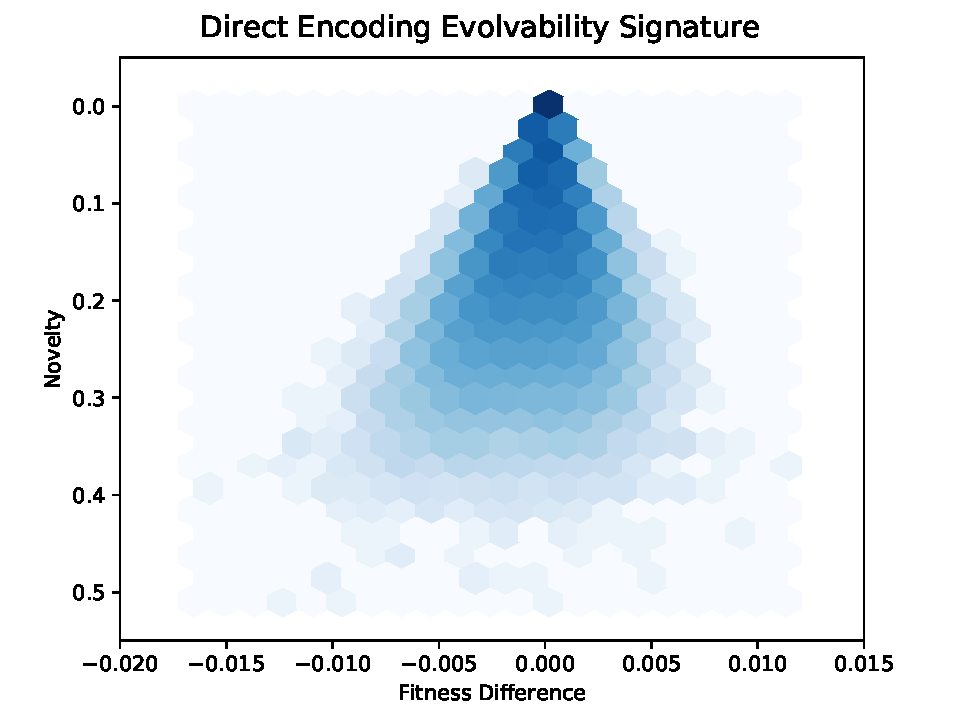
\includegraphics[width=\linewidth]{img/direct_es_unscaled}
    \subcaption{
      direct map
    }\label{fig:table_direct_es}
  \end{subfigure}
  \begin{subfigure}[b]{0.33\linewidth}
    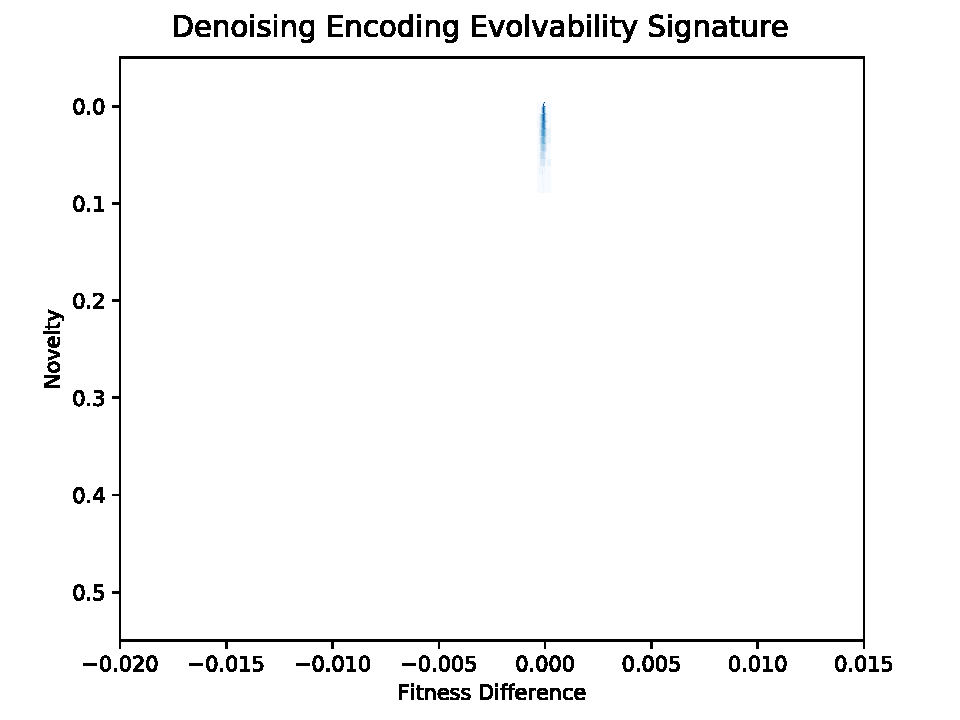
\includegraphics[width=\linewidth]{img/noise_es_unscaled}
    \subcaption{
      denoising map
    }\label{fig:table_noise_es}
  \end{subfigure}
  \begin{subfigure}[b]{0.33\linewidth}
    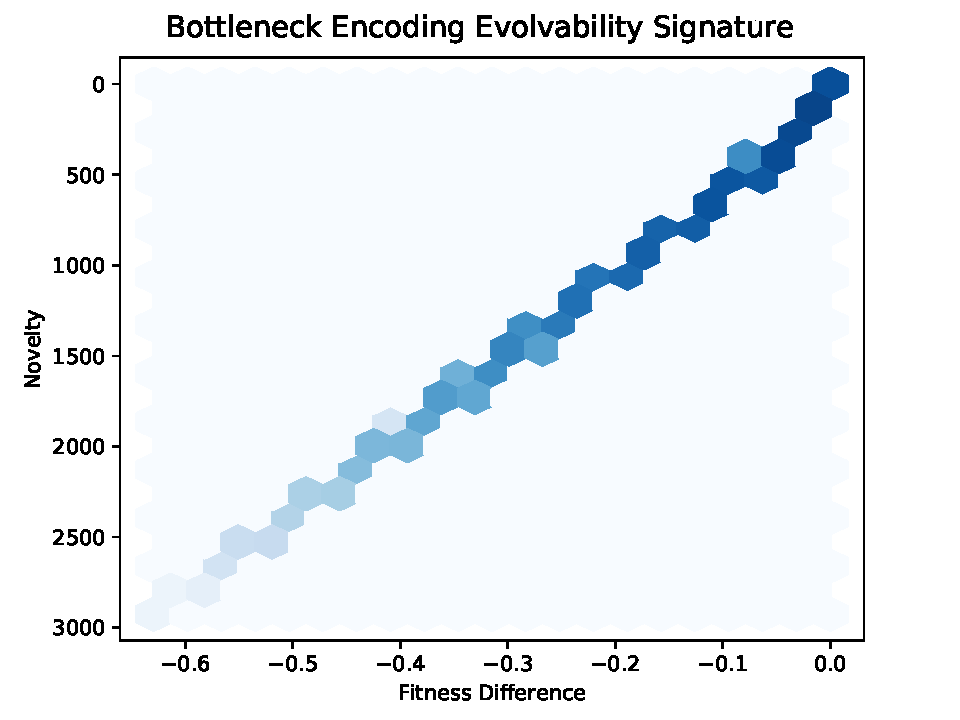
\includegraphics[width=\linewidth]{img/bottleneck_es_unscaled}
    \subcaption{
      bottleneck map
    }\label{fig:table_bottleneck_es}
  \end{subfigure}
  \caption{
    Evolvability signatures for three genotype-phenotype maps in the $n$-legged table problem domain.
    Note that subfigure \ref{fig:table_bottleneck_es} is presented with different axis scaling than subfigures \ref{fig:table_direct_es} and \ref{fig:table_noise_es}.
  }\label{fig:all_es}
\end{figure*}


Evolvability signature analysis was used to characterize the evolvability of the learned $n$-legged table bottleneck and denoiser encodings.
To generate these signatures, 20 replicate populations were evolved for 250 generations.
Then, the individual with the best fitness score over those 250 generations was isolated.
The novelty (euclidean distance between a parent phenotype and a child phenotype) and fitness scores of mutant offspring generated from that champion individual were used to create the evolvability signatures.
Figure \ref{fig:all_es} provides evolvability signatures for the direct, bottleneck, and denoiser genotype-phenotype maps.
It can clearly be seen that the bottleneck mapping can generate much more novelty per mutational step than either of the other mappings.
Fitness does decline in tandem with novelty, but the absolute fitness scores of nearly all offspring under the bottleneck mapping are greater than the absolute fitness of the direct-evolved champions (not shown).
Relatedly, although beneficial mutational outcomes are observed frequently under the direct encoding this is likely affected by relatively low absolute fitness of $-0.82$ ($s=0.1$) for direct-evolved champions (in comparison, for instance, to absolute fitness of $-0.025$, $s=0.004$ for denoiser-evolved champions).
Finally, more novelty is produced by mutation under the direct encoding compared to the denoising encoding.
The denoiser's action filtering out certain phenotypic variation likely contributes to observed the reduction of novelty observed under mutation.

Subsequently, we performed experiments to assess the ability of the three genotype-phenotype maps to facilitate traversal of the evolutionary search space in response to a selective pressure.
Specifically, a selective pressure for short (i.e. zero) table height was added.
Table height is calculated as the mean leg length of a table.
For each map, three replicate populations of 300 individuals were evolved for 5,000 generations.
These populations were initialized to have table height of approximately 1,000.
Response to selective pressure for short table height was assessed by tracking mean table height of the populations generation-by-generation.

\begin{figure}
  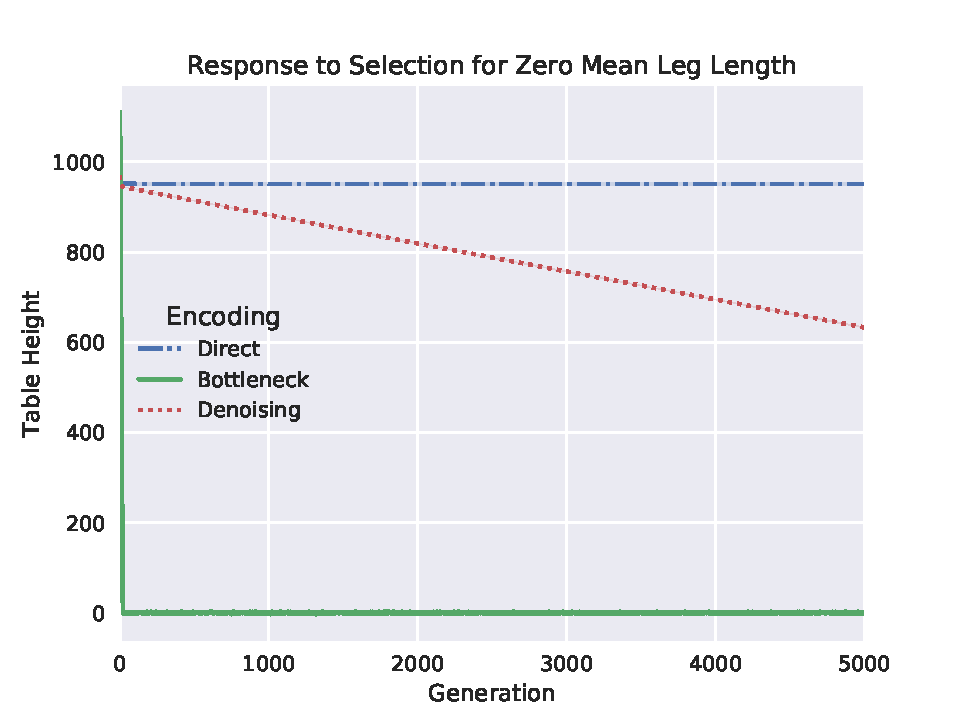
\includegraphics[width=\linewidth]{img/zero_leg_selection}
  \caption{Response to short-table selection pressure under different genotype-phenotype maps.}
  \label{fig:select_response}
\end{figure}


Figure \ref{fig:select_response} plots mean table height by generation under selection for both zero table height and table stability (described in detail in Section \ref{sec:methods}).
Shaded areas, hugging the table height trajectories so tight as to be difficult to discern, represent bootstrapped 95\% confidence intervals ($n=3$).

Under the direct mapping, a slight decrease in mean table height is observed for a few generations after initialization.
However, no further decrease in mean table height was observed over the course of evolutionary runs.
These runs ended with a mean table height of approximately 950.
Direct-encoded populations were trapped at local fitness peaks and unable to respond to selective pressure for short table height.

Under the bottleneck mapping, a severe decrease in mean table height is observed after initialization.
Well within 100 generations, the populations have come close to the global fitness peak --- a level table with height 0.
Populations with the bottleneck mapping were able to quickly respond to selective pressure for short table height.

Finally, under the denoising mapping, a slight drop-off in mean table height is observed after initialization.
Then, a steady decrease in table height was observed for the remainder of the evolutionary runs.
These runs ended with a mean table height of approximately 630.
Although not as swiftly as under the bottleneck mapping, under the denoising mapping populations were still able to respond to selective pressure for short table height.

Cursory inspection of input/output of the decoding component of the bottleneck autoencoder revealed that it had learned to echo the single bottlenecked float in order to uniformly populate the vector of 100 phenotypic leg lengths.
Thus, the bottleneck genetic representation essentially described the table height; table leg lengths were set using this height value via the genotype-phenotype map.
Evolvability signature analysis suggests that this encoding allows the generation of greater novelty with less deleterious consequence.
Indeed, as in Figure \ref{fig:select_response}, table populations using this encoding are able to rapidly evolve to a global fitness peak.
Similar inspection of the denoising autoencoder revealed that that neural network had essentially learned to calculate each phenotypic leg length output as the average of its inputs.
Thus, the denoising encoding took genetic input for what --- under the direct encoding --- would otherwise be an unstable table and output a stable table nearby in phenotype space.
Evolvability signature analysis shows that although this encoding does not enhance the novelty of phenotypic outcomes under mutation relative to the direct encoding, it does curb the deleterious effects of mutation.
Thus, as in Figure \ref{fig:select_response}, table populations using this encoding are able to make slow and steady progress towards a global fitness peak.

\subsection{Scrabble String Problem}

\begin{figure}
  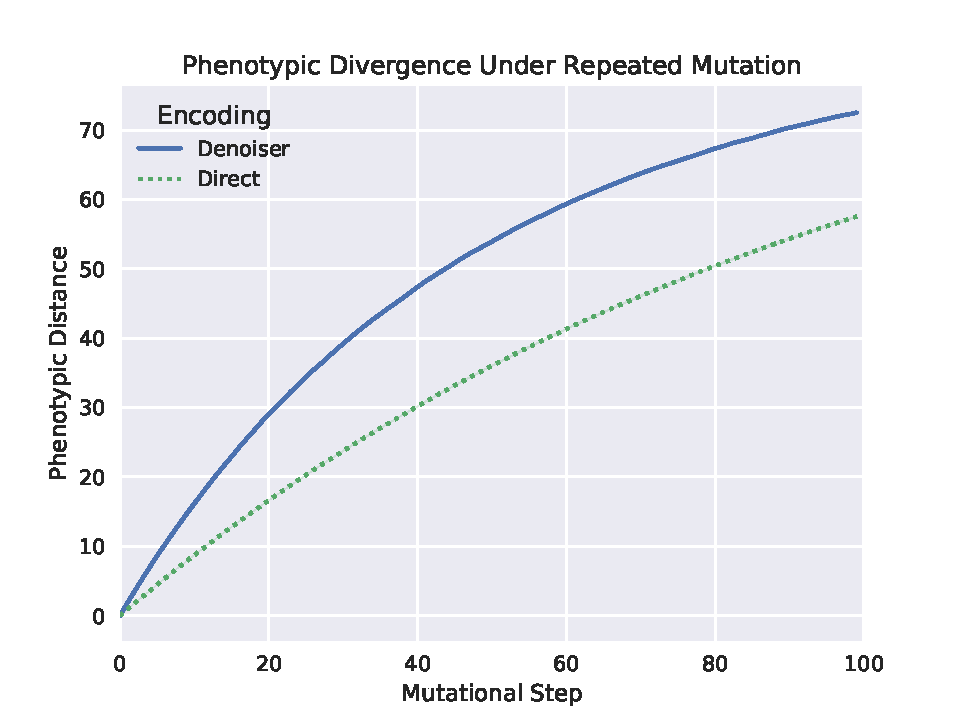
\includegraphics[width=\linewidth]{img/scrabble_dist_vs_step}
  \caption{TODO}
  \label{fig:scrabble_dist_vs_step}
\end{figure}

\begin{figure}
  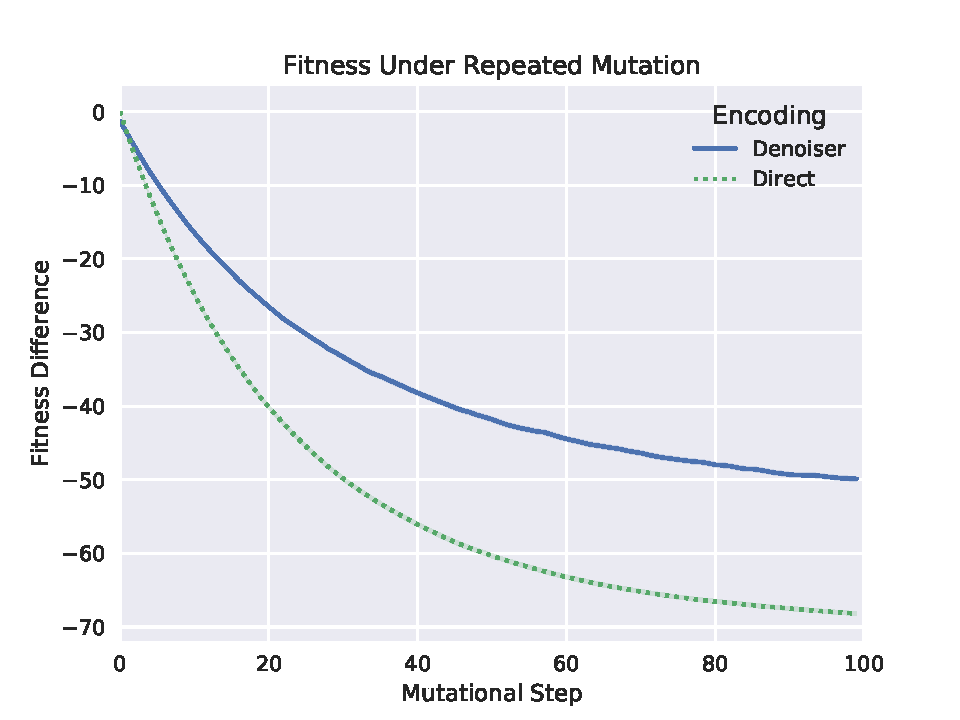
\includegraphics[width=\linewidth]{img/scrabble_fit_diff_vs_step}
  \caption{Fitness loss by mutational step in the Scrabble string domain.}
  \label{fig:scrabble_fit_diff_vs_step}
\end{figure}

\begin{figure}
  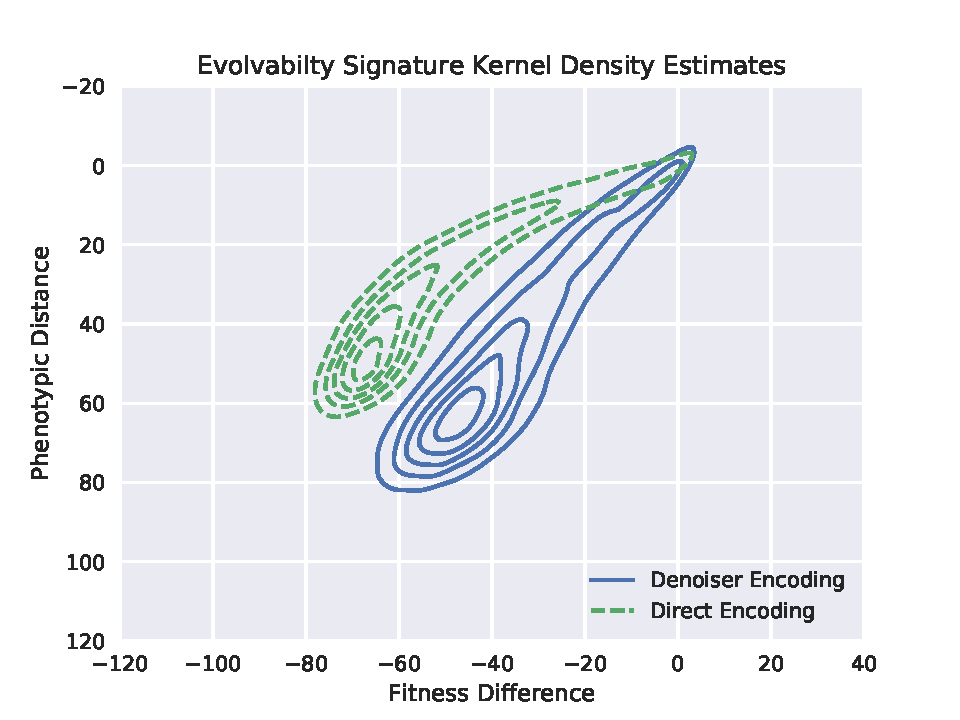
\includegraphics[width=\linewidth]{img/scrabble_es_kde}
  \caption{Gaussian kernel density estimates for evolvability signatures of direct and indirect encodings in Scrabble string domain.}
  \label{fig:scrabble_es_kde}
\end{figure}

\begin{figure}
  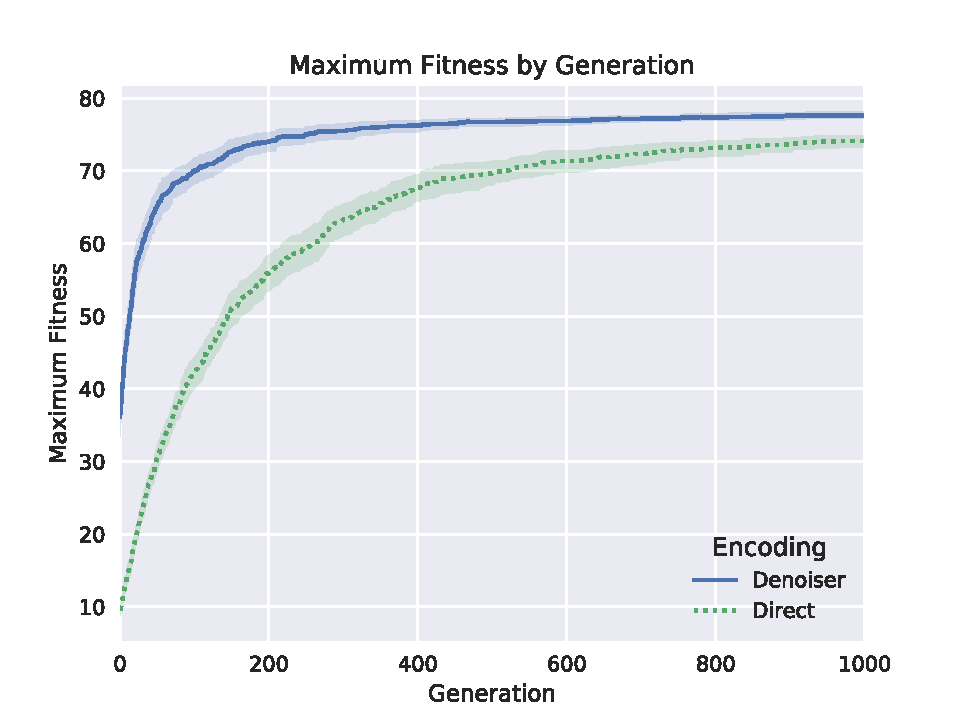
\includegraphics[width=0.8\linewidth]{img/scrabble_fit_vs_gen}
  \caption{
    Maximum individual fitness by generation in populations evolving in the Scrabble string domain.
  }\label{fig:scrabble_fit_vs_gen}
\end{figure}


Evolvability signature analysis was used to characterize the evolvability of the learned denoiser encoding in the scrabble string.
To generate these signatures, 250 champion genotypes were drawn from the direct-encoded populations used to train the denoiser encoding.
100-step mutational walks were then taken from the champion genotype.
The phenotypes generated from those genotypes under both the direct and the denoising encoding were compared.
Figure \ref{fig:scrabble_dist_vs_step} plots novelty (number of non-matching phenotypic characters between the original champion and its mutant offspring) against mutational step ($n=250$).
Novelty increases more rapidly under the denoiser encoding relative to the direct encoding.
Figure \ref{fig:scrabble_fit_diff_vs_step} plots fitness relative to the original champion against mutational step ($n=250$).
Fitness declines more slowly under mutation with the denoiser encoding compared to the direct encoding.
In both of these figures, bootstrapped 95\% confidence are shaded along each curve but are tight enough to be difficult to discern.
Figure \ref{fig:scrabble_es_kde} ties together fitness and novelty information from these random mutational walks in the format of an evolvability signature.
Kernel density estimates contours of evolvability signature densities under both encodings are shown side-by-side.
From this comparison, it seems that the denoiser encoding simultaneously yields more novelty and less fitness decline under mutation.

Subsequently, we tested the capacity of the denosier encoding to speed up adaptive evolution.
We set up twenty replicate Scrabble string populations to use the the denoiser genotype-phenotype map and twenty Scrabble string populations to use the direct map.
For each population, maximum fitness was recorded over 1,000 generations of evolution.
Figure \ref{fig:scrabble_fit_vs_gen} shows that the populations using the denoiser encoding gain fitness at a much quicker rate than the direct encoding over the first few hundred generations ($n=20$).
(Again, bootstrapped 95\% confidence are shaded along each curve.)
Clearly, the evolvability properties of the denoiser encoding translate to evolutionary dynamics that differ strongly from the direct encoding.

As shown in Figure \ref{fig:scrabble_denoiser}, the denoising autoencoder revealed that it had essentially learned to spell-check a genotype to generate the phenotype.
Generally, though not always, characters part of valid words are left undisturbed.
Interestingly, the change that the denoiser makes to correct a spelling error doesn't always reflect the original state of the string.
There are often several possible repairs that will yield valid spelling outcomes.
We hypothesize that this dynamic explains the rapid rate of novelty increase under mutation --- often, instead of correcting the mutated site in the phenotype corrections are applied to one or several \textit{other} sites.
Thus, more than one character in the phenotype may change due to mutation of a single site in the genome.
In particular, based on informal analysis of example sentences fed to it, the denoising autoencoder seems to somewhat favor fixing spelling mistakes by strategically replacing a letter character with a space.
This might occur because the denoiser encountered spaces more often than any other single character during training.
